%!TEX program = pdflatex

\documentclass[a4paper, 12pt]{article}

\usepackage{geometry}
\geometry{a4paper,
total={170mm,257mm},left=2cm,right=2cm,
top=1cm,bottom=2cm}

\usepackage{mathtext}
\usepackage{amsmath}
\usepackage[T2A]{fontenc}
\usepackage[utf8]{inputenc}
\usepackage[english,russian]{babel}
\usepackage{graphicx, float}
\usepackage{tabularx, colortbl}
\usepackage{caption}
\captionsetup{labelsep=period}

\newcommand{\parag}[1]{\paragraph*{#1:}}
\DeclareSymbolFont{T2Aletters}{T2A}{cmr}{m}{it}
\newcounter{Points}
\setcounter{Points}{1}
\newcommand{\point}{\arabic{Points}. \addtocounter{Points}{1}}
\newcolumntype{C}{>{\centering\arraybackslash}X}

\author{Костылев Владислав и Шатров Игорь, Б01-206}
\date{\today}
\title{Отчет о выполнении лабораторной работы 5.1.2 \\ \textbf{Эффект Комптона} }

\begin{document}
%\maketitle

\begin{titlepage}
		\vspace*{\fill}
		
		\begin{center}
			
\includegraphics[scale=0.8]{res/MIPT.pdf}
			\\[0.7cm]\Huge Московский Физико-Технический Институт
			\\[2cm]\LARGE Отчет о выполнении лабораторной работы 
			\\[0.5cm]\noindent\rule{\textwidth}{1pt}
			\\\Huge\textbf{5.1.2 \\ Эффект Комптона}
			\\[-0.5cm]\noindent\rule{\textwidth}{1pt}
		\end{center}
		
		\vspace*{\fill}
		
		\begin{flushleft}
			Выполнили: \hspace{\fill} Группа:
			\\Костылев Владислав \\ Шатров Игорь \hspace{\fill} Б01-206
		\end{flushleft}
	\end{titlepage}

	\setcounter{page}{2}

\begin{abstract}
    \textbf{Цель работы:}
    С помощью сцинтилляционного спектрометра исследуется энергетический спектр $\gamma$ - квантов, 
    рассеянных на графите. Определяется энергия рассеянных $\gamma$ -квантов в зависимости от угла рассеяния, 
    а также энергия покоя частиц, на которых происходит комптоновское рассеяние.
\end{abstract}

\tableofcontents
\newpage

\section{Введение} 
    Рассеяние $\gamma$ -лучей в веществе относится к числу явлений, 
    в которых особенно ясно проявляется двойственная природа излучения. 
    Волновая теория, хорошо объясняющая рассеяние длинноволнового излучения, 
    испытывает трудности при описании рассеяния рентгеновских и $\gamma$ -лучей. 
    Эта теория, в частности, не может объяснить, почему в составе рассеянного излучения, 
    измеренного Комптоном, кроме исходной волны с частотой $\omega_{0}$ появляется дополнительная длинноволновая компонента, 
    отсутствующая в спектре первичного излучения.

    Появление этой компоненты легко объяснимо, если считать, что $\gamma$-излучение представляет собой поток квантов (фотонов), 
    имеющих энергию $\hbar \omega$ и импульс $p=\hbar \omega / c .$ 
    Эффект Комптона - увеличение длины волны рассеянного излучения по сравнению с падающим - интерпретируется 
    как результат упругого соударения двух частиц: $\gamma$ -кванта (фотона) и свободного электрона.

    Рассмотрим элементарную теорию эффекта Комптона. 
    Пусть электрон до соударения покоился (его энергия равна энергии покоя $m c^{2}$ ), 
    a $\gamma$ -квант имел начальную энергию $\hbar \omega_{0}$ и импульс $\hbar \omega_{0} / c .$ 
    После соударения электрон приобретает энергию $\gamma m c^{2}$ и импульс $\gamma m v,$ 
    где $\gamma=\left(1-\beta^{2}\right)^{-1 / 2}, \beta=v / c,$ a $\gamma$ -квант рассеивается 
    на некоторый угол $\theta$ по отношению к первоначальному направлению движения. 
    Энергия и импульс $\gamma$ -кванта становятся соответственно равным 
    и $\hbar \omega_{1}$ и $\hbar \omega_{1} / c$. 
   
    Запишем для рассматриваемого процесса законы сохранения энергии и импульса:
    \[
        \begin{array}{c}
            m c^{2}+\hbar \omega_{0}=\gamma m c^{2}+\hbar \omega_{1} \\
            \frac{\hbar \omega_{0}}{c}=\gamma m v \cos \varphi+\frac{\hbar \omega_{1}}{c} \cos \theta \\
            \gamma m v \sin \varphi=\frac{\hbar \omega_{1}}{c} \sin \theta
        \end{array}
    \]

    Решая совместно эти уравнения и переходя от частот $\omega_{0}$ и $\omega_{1}$ 
    к длинам волн $\lambda_{0}$ и $\lambda_{1},$ нетрудно получить, что изменение длины волны рассеянного излучения равно
    \begin{equation}
    \Delta \lambda=\lambda_{1}-\lambda_{0}=\frac{h}{m c}(1-\cos \theta)=\Lambda_{\mathrm{K}}(1-\cos \theta)
    \end{equation}
    где $\lambda_{0}$ и $\lambda_{1}$ - длины волн $\gamma$ -кванта до и после рассеяния, а величина
    \[
        \Lambda_{\mathrm{K}}=\frac{h}{m c}=2,42 \cdot 10^{-10} \mathrm{cm}
    \]

    Основной целью данной работы является проверка соотношения
    (1). Применительно к условиям нашего опыта формулу
    (1) следует преобразовать от длин волн к энергии $\gamma$ -квантов. 
    Как нетрудно показать, соответствующее выражение имеет вид
    \begin{equation}
        \frac{1}{\varepsilon(\theta)}-\frac{1}{\varepsilon_{0}}=1-\cos \theta
    \end{equation}
    
    Здесь $\varepsilon_{0}=E_{0} /\left(m c^{2}\right)-$ выраженная в единицах $m c^{2}$ энергия $\gamma$ -квантов, 
    падающих на рассеиватель, $\varepsilon(\theta)$ - выраженная в тех же единицах энергия квантов, 
    испытавших комптоновское рассеяние на угол $\theta, m-$ масса электрона.

\section{Экспериментальная установка}
    Блок-схема установки изображена на рисунке ниже. 
    
    \begin{figure}[H]
        \centering
        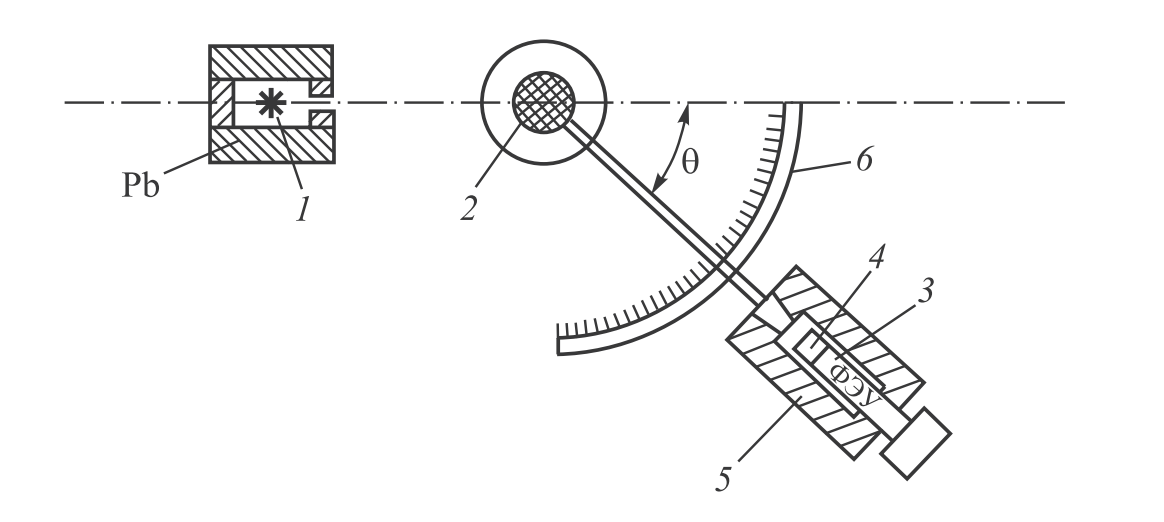
\includegraphics[width=0.7\linewidth]{res/1.png}
    \end{figure}

    Источником излучения 1 служит $137 \mathrm{Cs},$ испускающий $\gamma$ -лучи с энергией 662 кэВ. 
    Он помещен в толстостенный свинцовый контейнер с коллиматором. 
    Сформированный коллиматором узкий пучок $\gamma$ -квантов попадает 
    на графитовую мишень 2 (цилиндр диаметром 40 мм и высотой 100 мм).
        
    Кванты, испытавшие комптоновское рассеяние в мишени, регистрируются сцинтилляционным счетчиком. 
    Счетчик состоит из фотоэлектронного умножителя 3 (далее ФЭУ) и сцинтиллятора 4. 
    Сцинтиллятором служит кристалл NaI(Tl) цилиндрической формы диаметром 40 мм и высотой 40 мм, 
    его выходное окно находится в оптическом контакте с фотокатодом ФЭУ. 
    Сигналы, возникающие на аноде ФЭУ, подаются на ЭВМ для амплитудного анализа. 
    Кристалл и ФЭУ расположены в светонепроницаемом блоке, укрепленном на горизонтальной штанге.     

% \section {Методика измерений}
    
    
\section{Результаты измерений и обработка данных} 

Для обработки результатов используется формула $(2)$ с замененными энергиями квантов на $N(\theta)$.
\begin{equation}
    \frac{1}{N(\theta)} - \frac{1}{N(0)} = A(1-\cos\theta)
\end{equation}

Далее, устанавливая сцинтилляционный датчик под разными углами мы получаем картины пиков, 
по которым мы измеряем уже номера каналов, в которых пик:

    \begin{figure}[H]
        \centering
        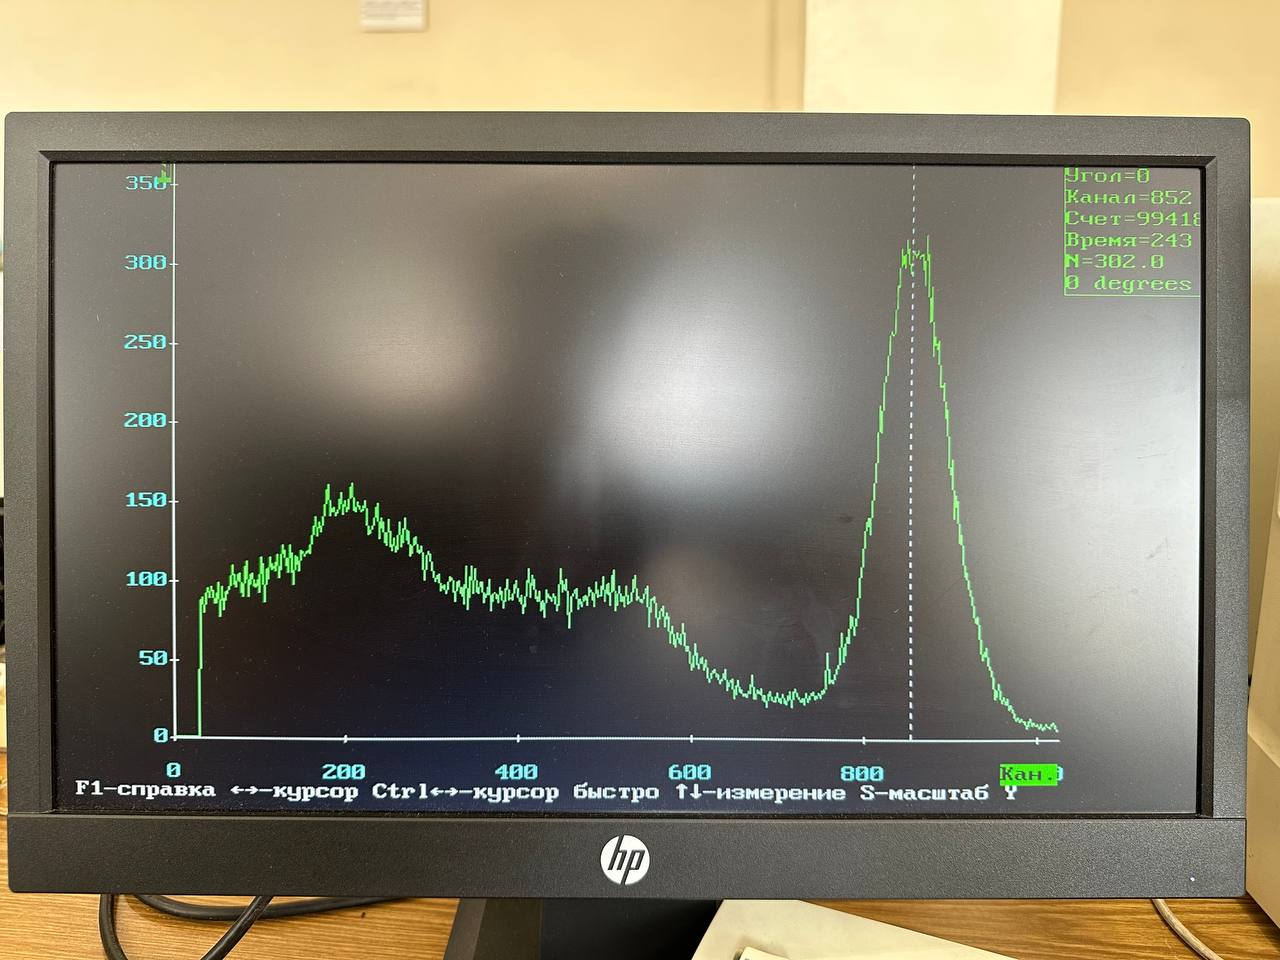
\includegraphics[width = 0.6\linewidth]{res/01.jpg}
        \caption{$\theta = 0^0$}
    \end{figure}

    \begin{figure}[H]
    \begin{minipage}[h]{0.3\linewidth}
        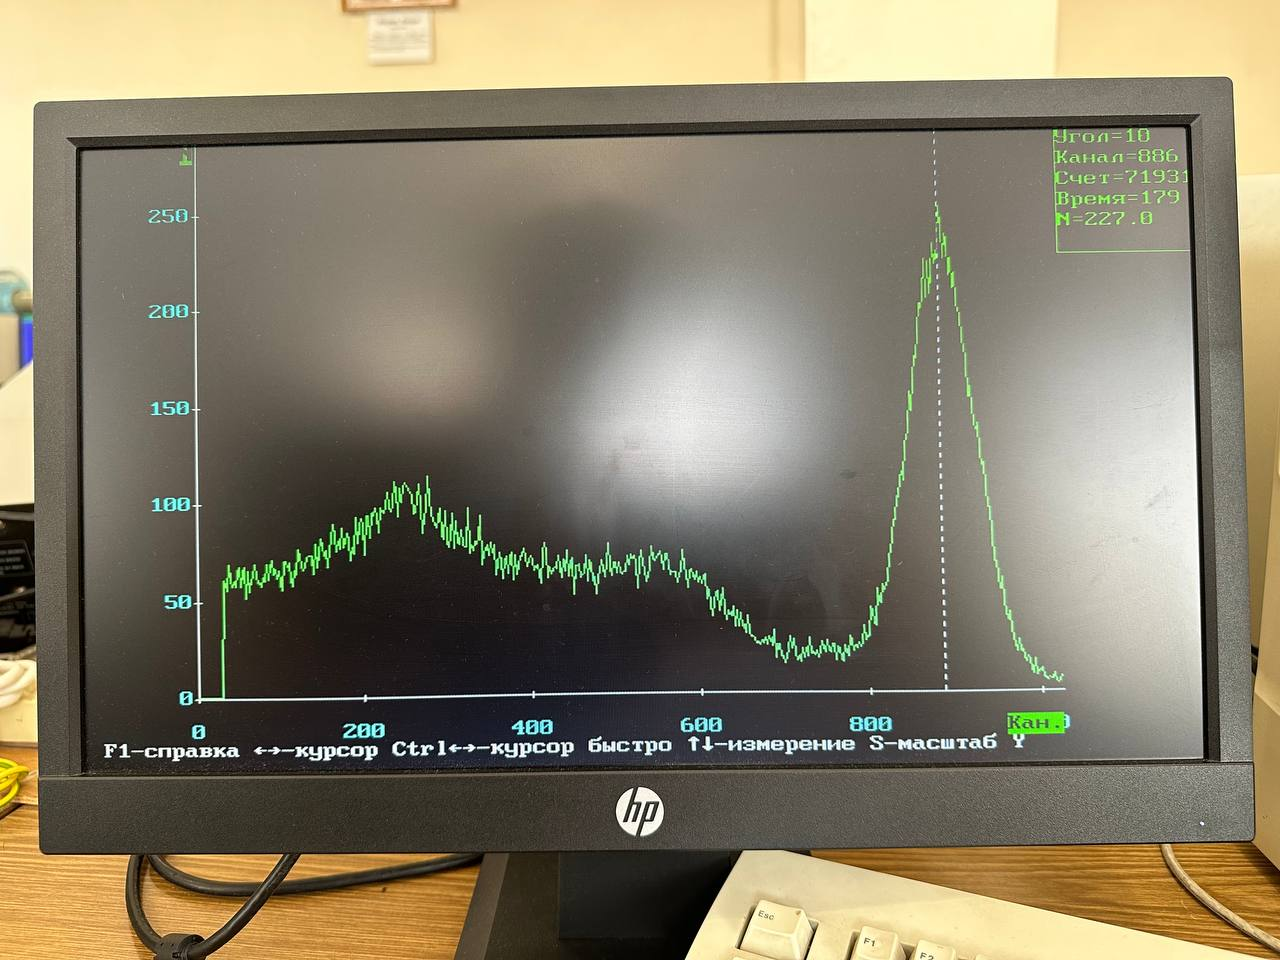
\includegraphics[width = 1\linewidth]{res/02.jpg}
        \caption{$\theta = 10^0$}
    \end{minipage}
    \hfill
    \begin{minipage}[h]{0.3\linewidth}
        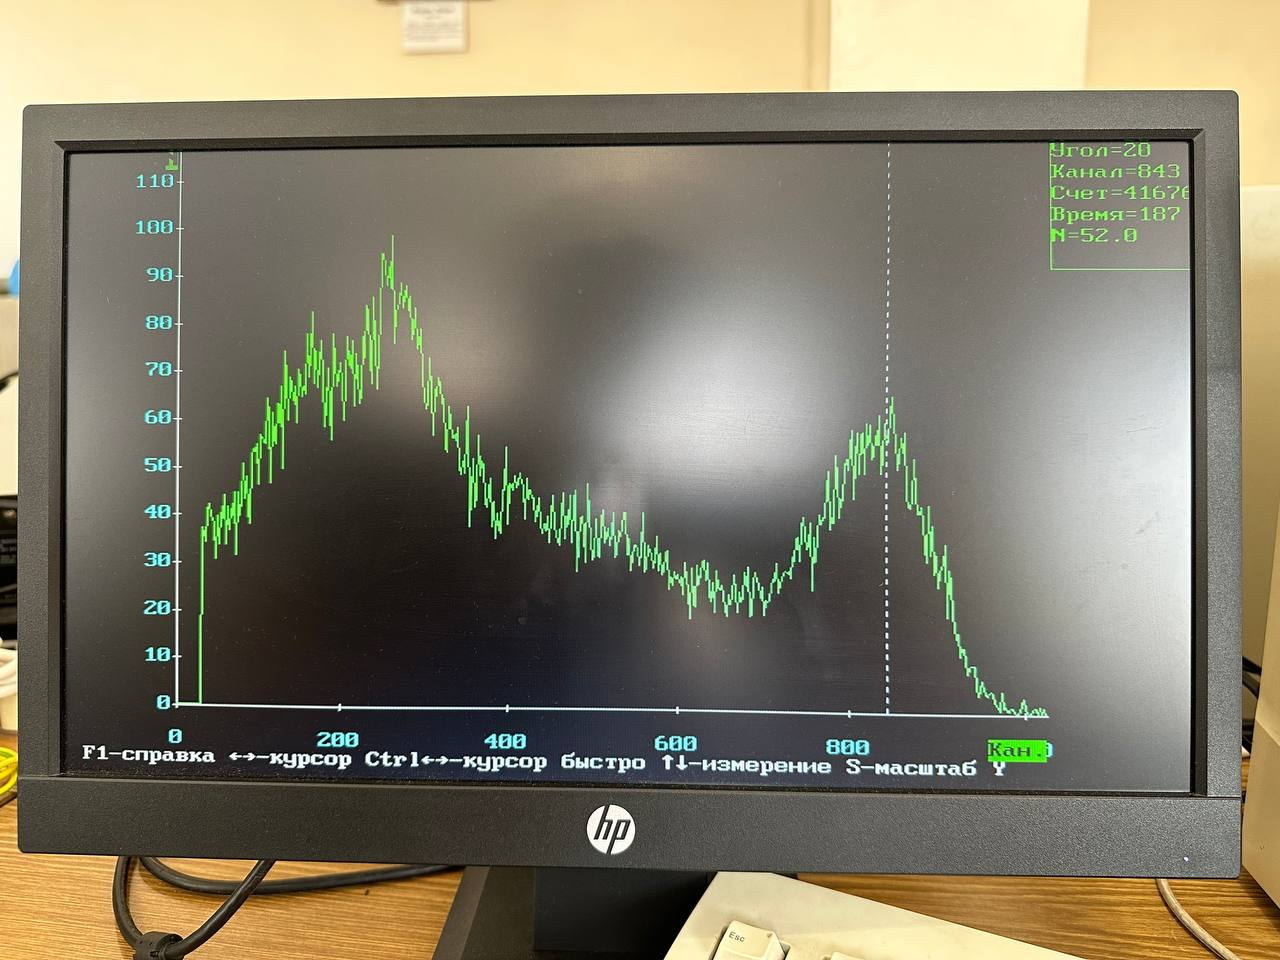
\includegraphics[width = 1\linewidth]{res/03.jpg}
        \caption{$\theta = 20^0$}
    \end{minipage}
    \hfill
    \begin{minipage}[h]{0.3\linewidth}
        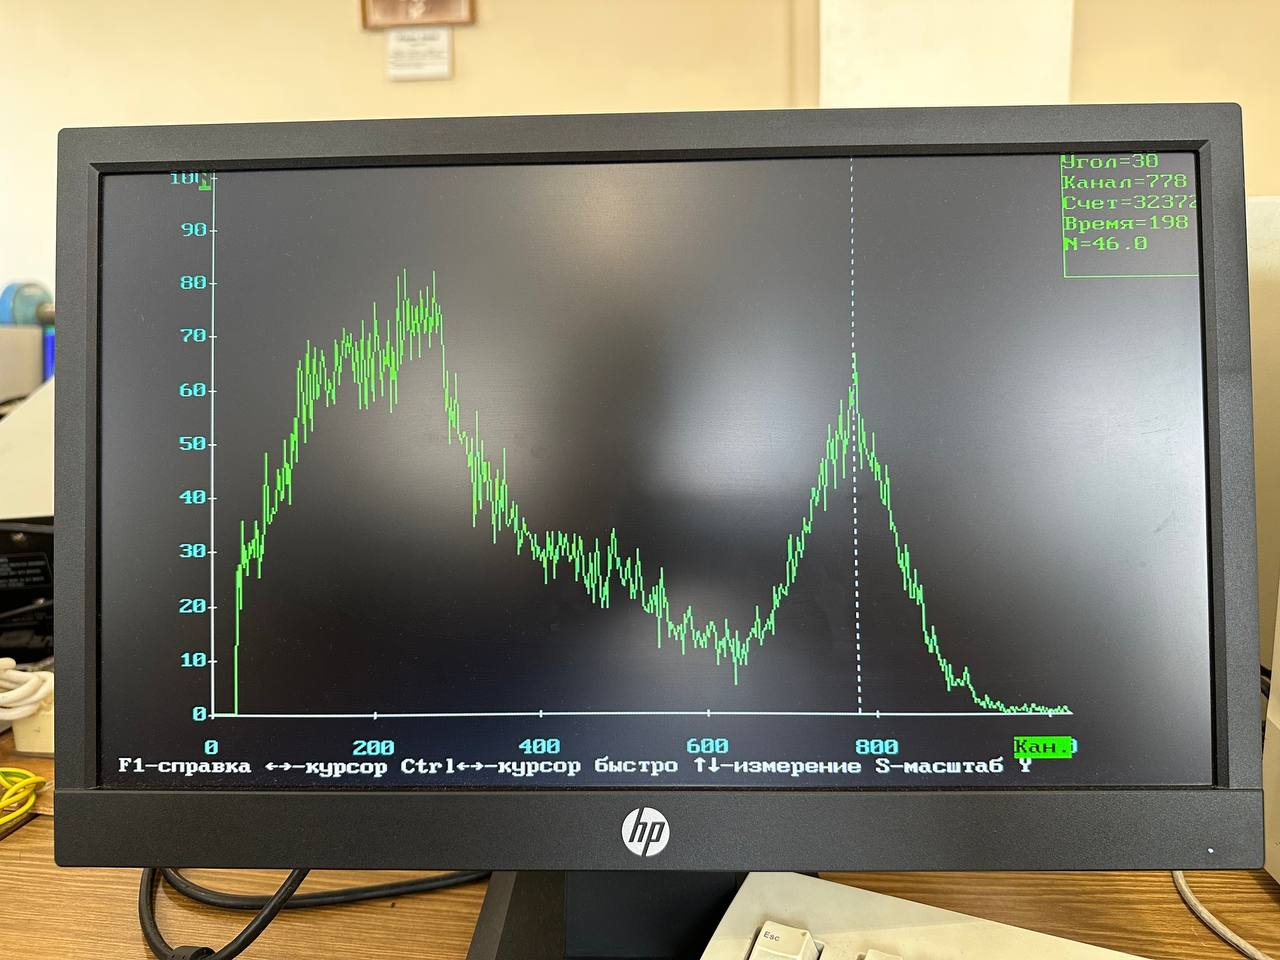
\includegraphics[width = 1\linewidth]{res/04.jpg}
        \caption{$\theta = 30^0$}
    \end{minipage}
    \end{figure}

    \begin{figure}[H]
    \begin{minipage}[h]{0.3\linewidth}
        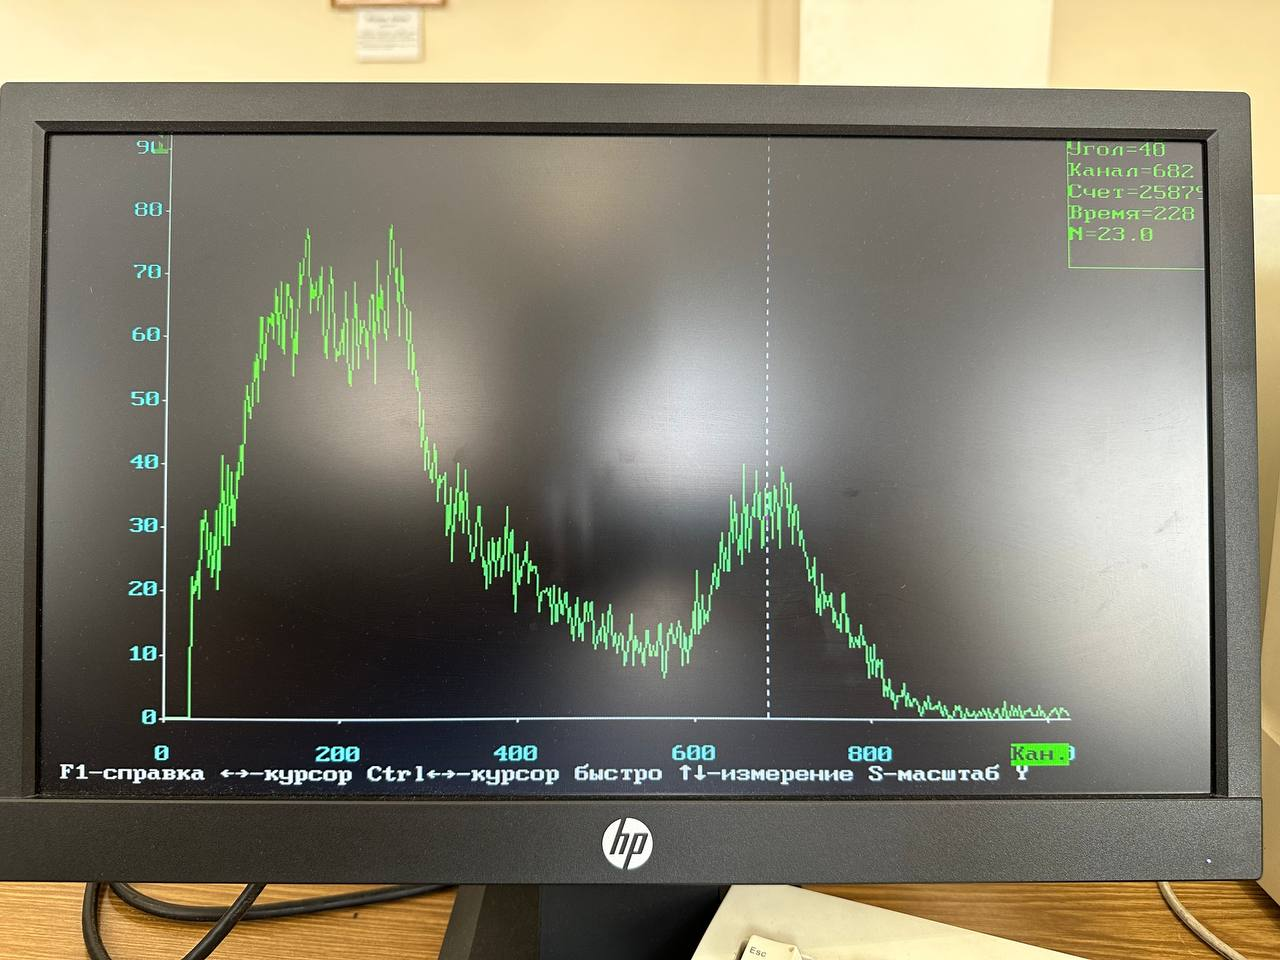
\includegraphics[width = 1\linewidth]{res/05.jpg}
        \caption{$\theta = 40^0$}
    \end{minipage}
    \hfill
    \begin{minipage}[h]{0.3\linewidth}
        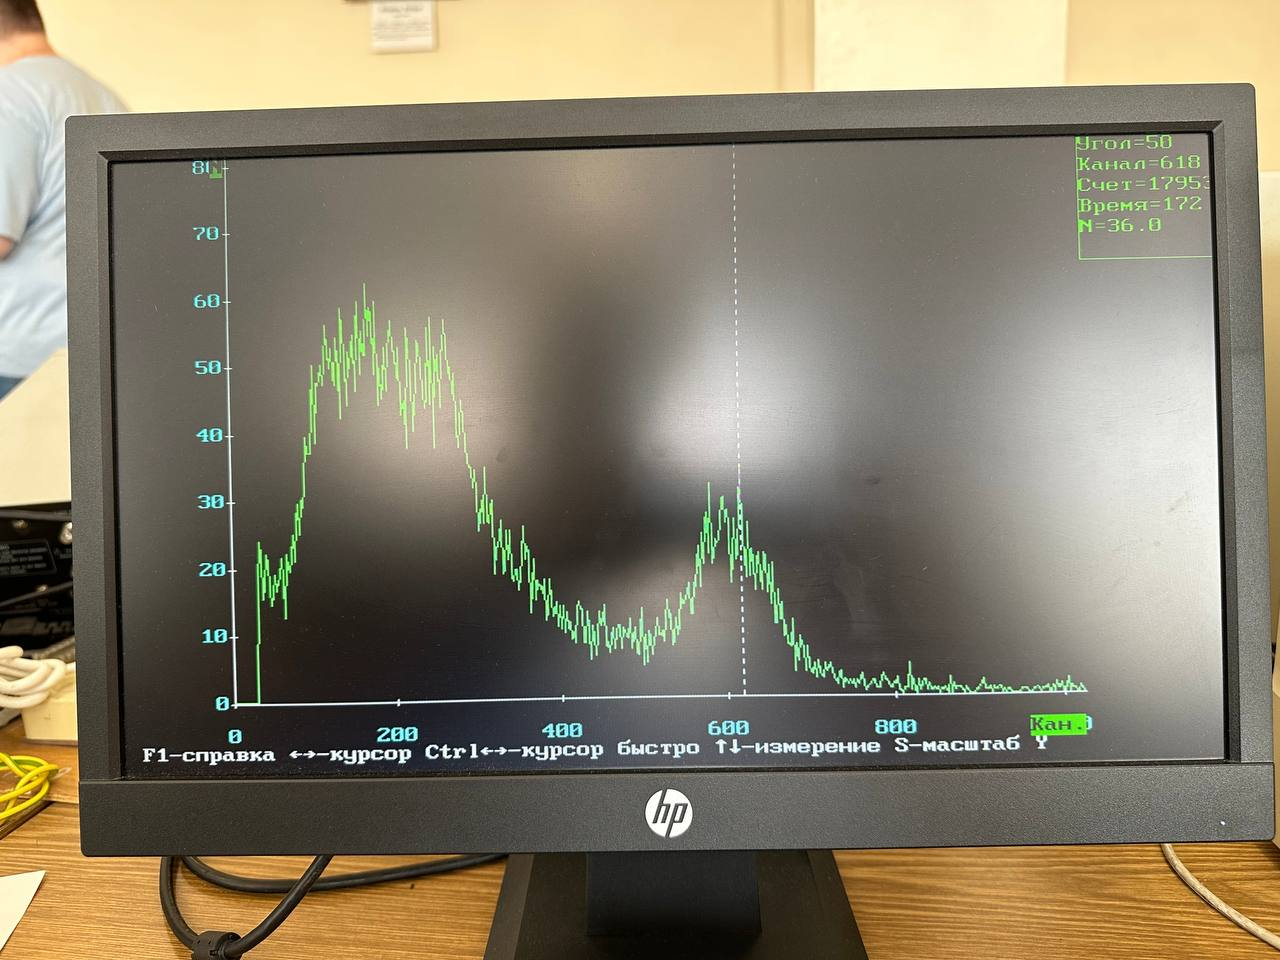
\includegraphics[width = 1\linewidth]{res/06.jpg}
        \caption{$\theta = 50^0$}
    \end{minipage}
    \hfill
    \begin{minipage}[h]{0.3\linewidth}
        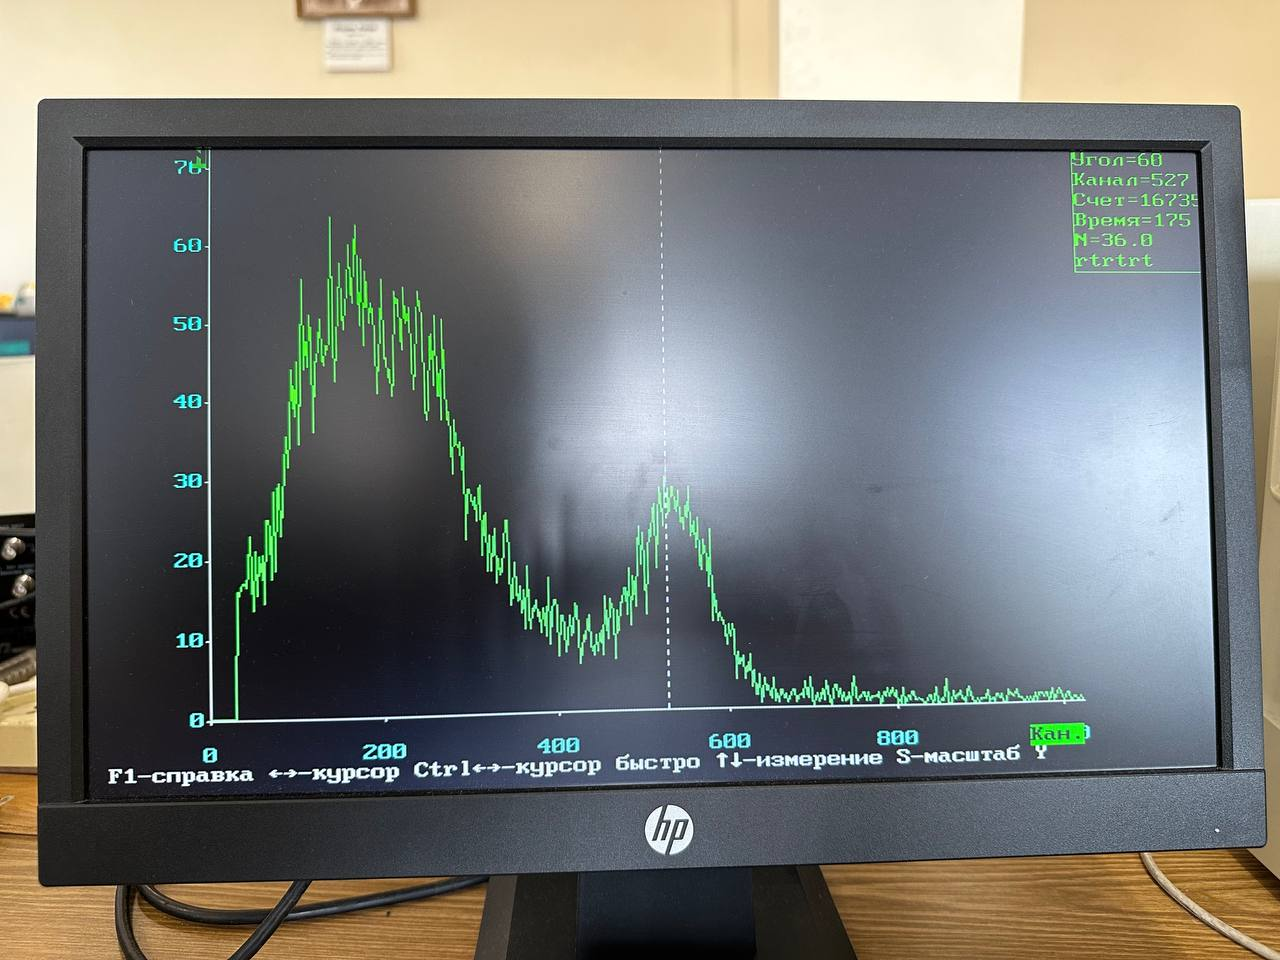
\includegraphics[width = 1\linewidth]{res/07.jpg}
        \caption{$\theta = 60^0$}
    \end{minipage}
    \end{figure}

    \begin{figure}[H]
    \begin{minipage}[h]{0.3\linewidth}
        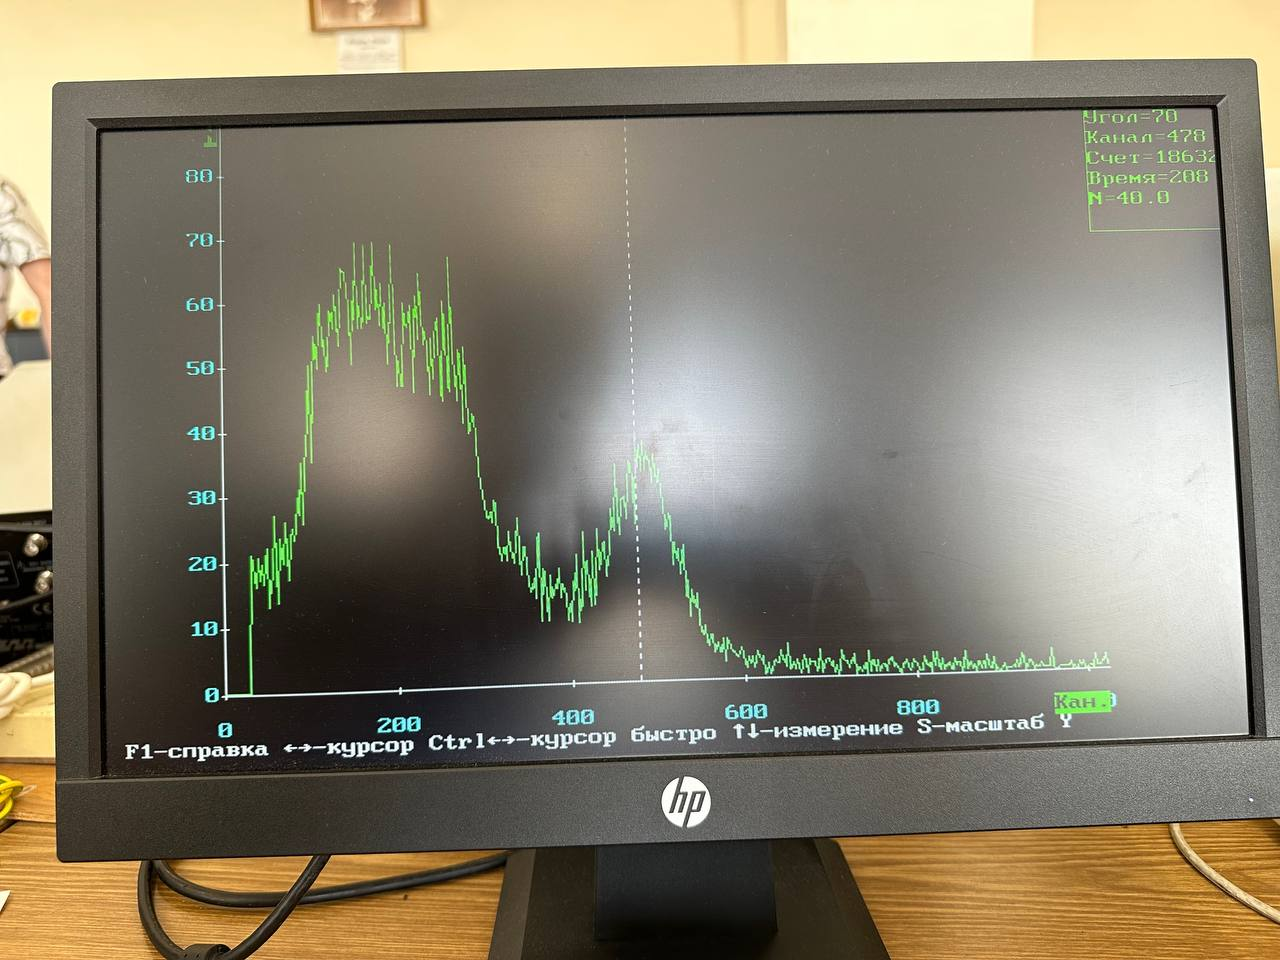
\includegraphics[width = 1\linewidth]{res/08.jpg}
        \caption{$\theta = 70^0$}
    \end{minipage}
    \hfill
    \begin{minipage}[h]{0.3\linewidth}
        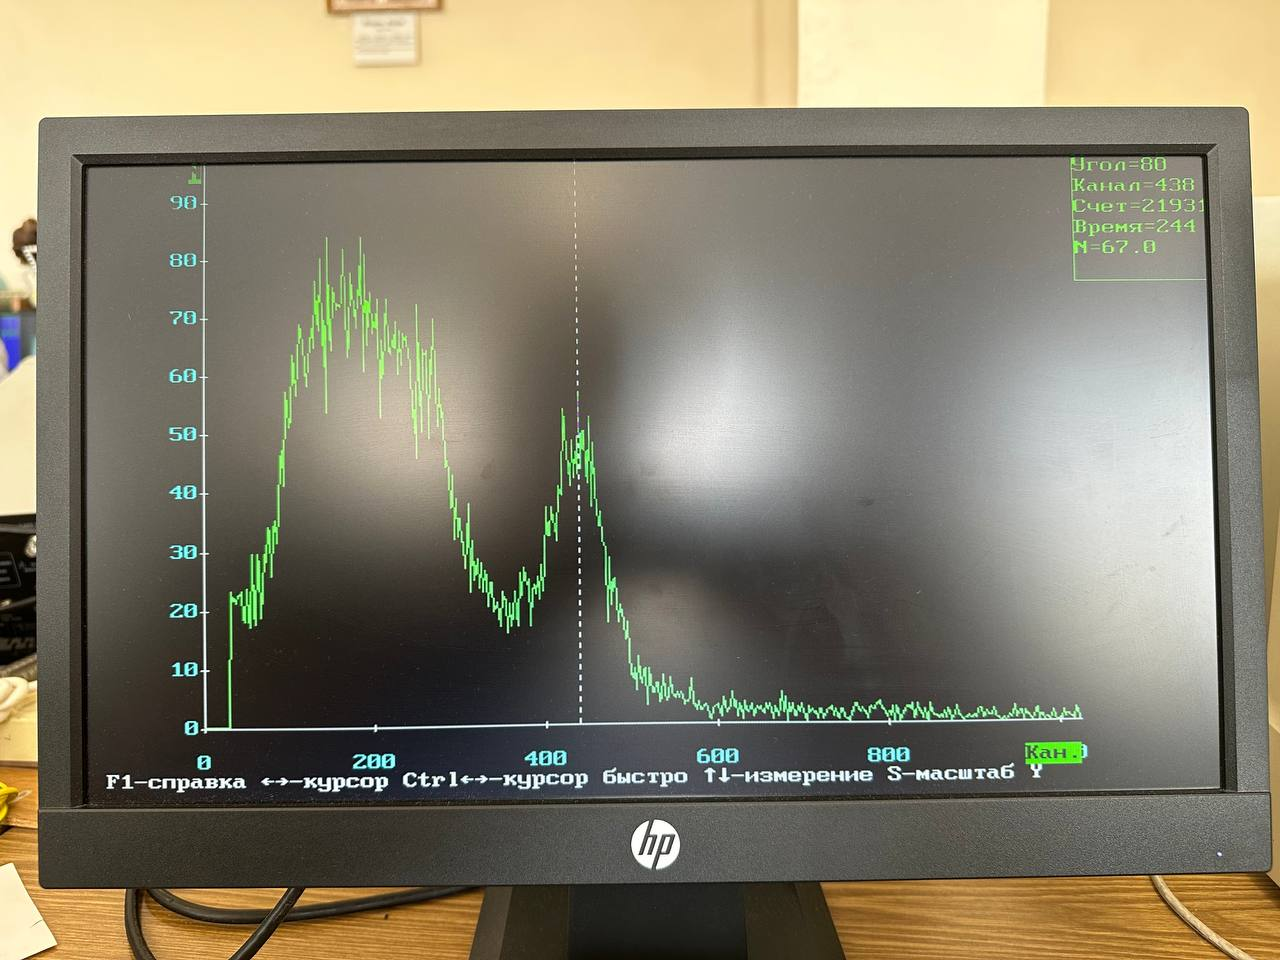
\includegraphics[width = 1\linewidth]{res/09.jpg}
        \caption{$\theta = 80^0$}
    \end{minipage}
    \hfill
    \begin{minipage}[h]{0.3\linewidth}
        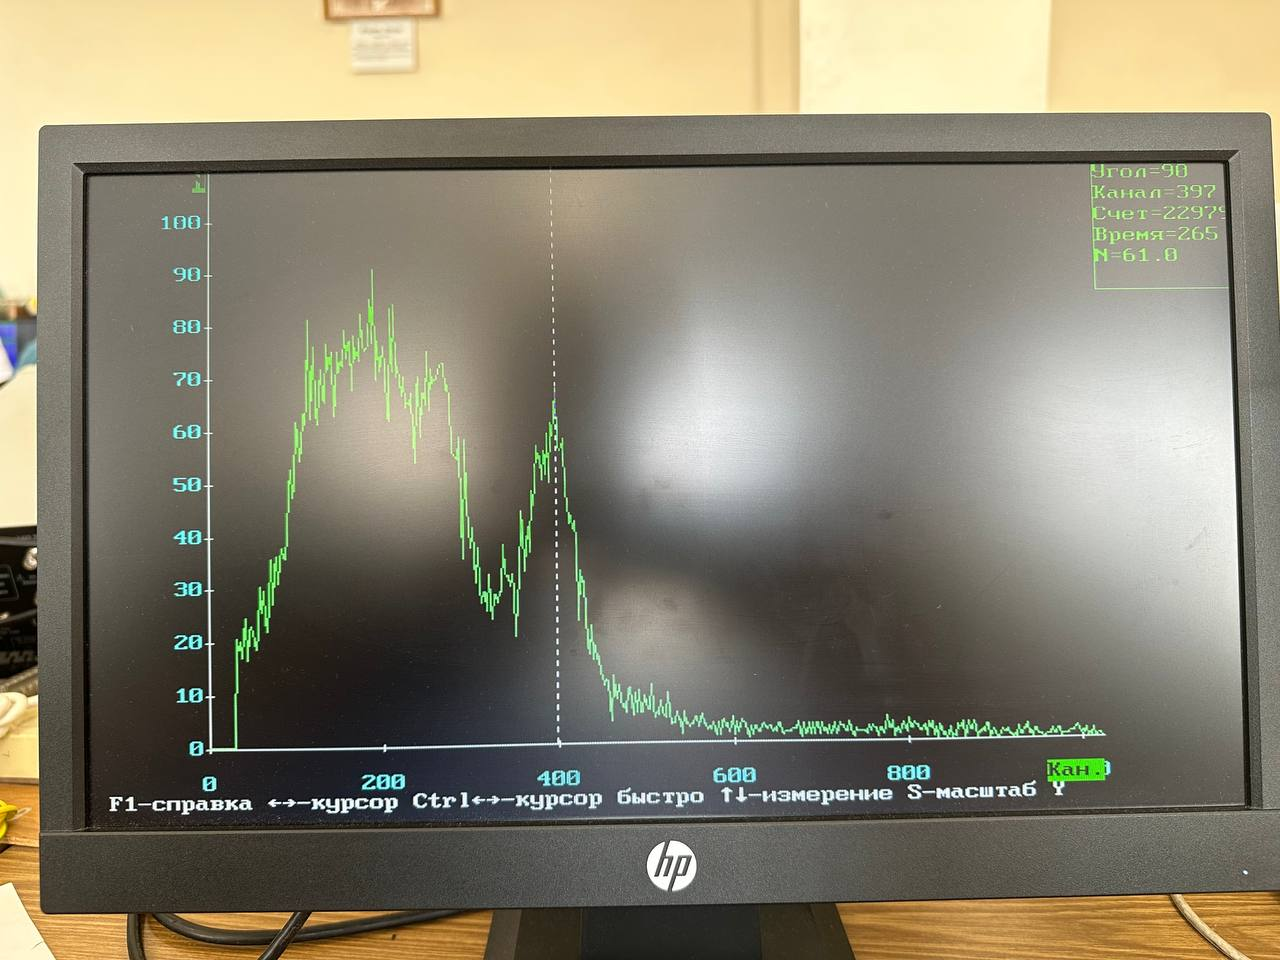
\includegraphics[width = 1\linewidth]{res/010.jpg}
        \caption{$\theta = 90^0$}
    \end{minipage}
    \end{figure}
    
    \begin{figure}[H]
    \begin{minipage}[h]{0.3\linewidth}
        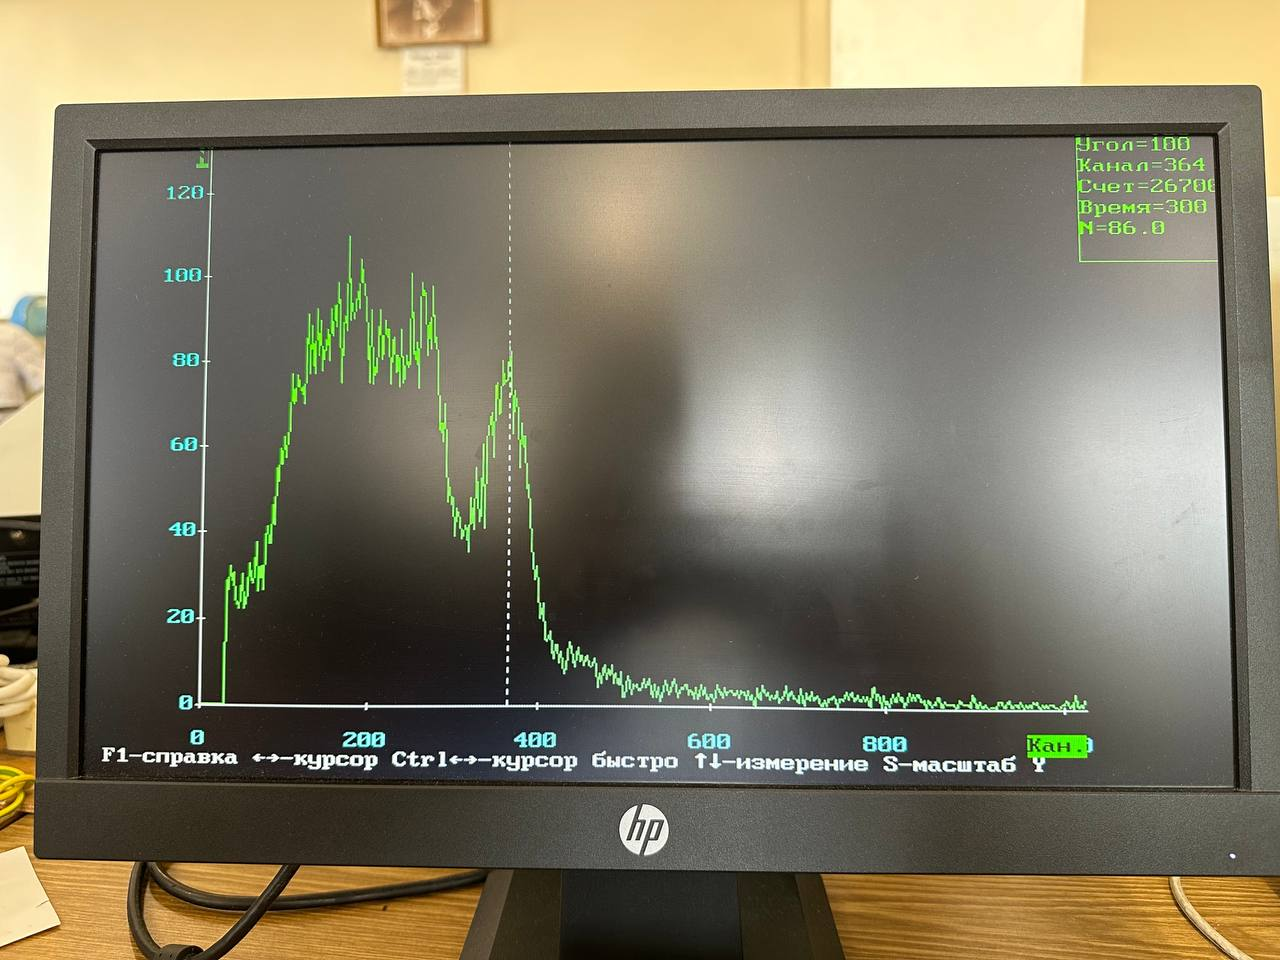
\includegraphics[width = 1\linewidth]{res/011.jpg}
        \caption{$\theta = 100^0$}
    \end{minipage}
    \hfill
    \begin{minipage}[h]{0.3\linewidth}
        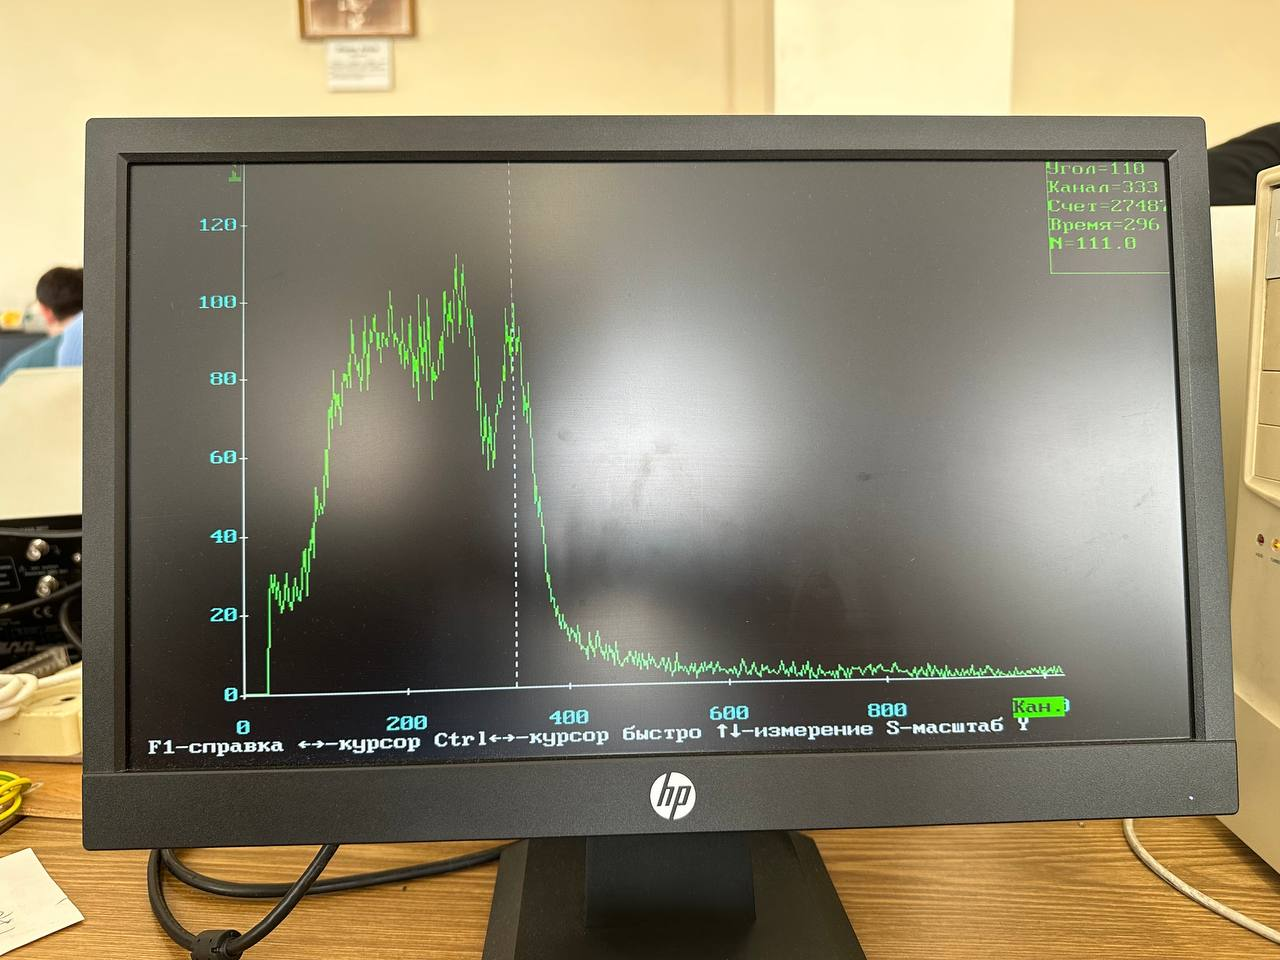
\includegraphics[width = 1\linewidth]{res/012.jpg}
        \caption{$\theta = 110^0$}
    \end{minipage}
    \hfill
    \begin{minipage}[h]{0.3\linewidth}
        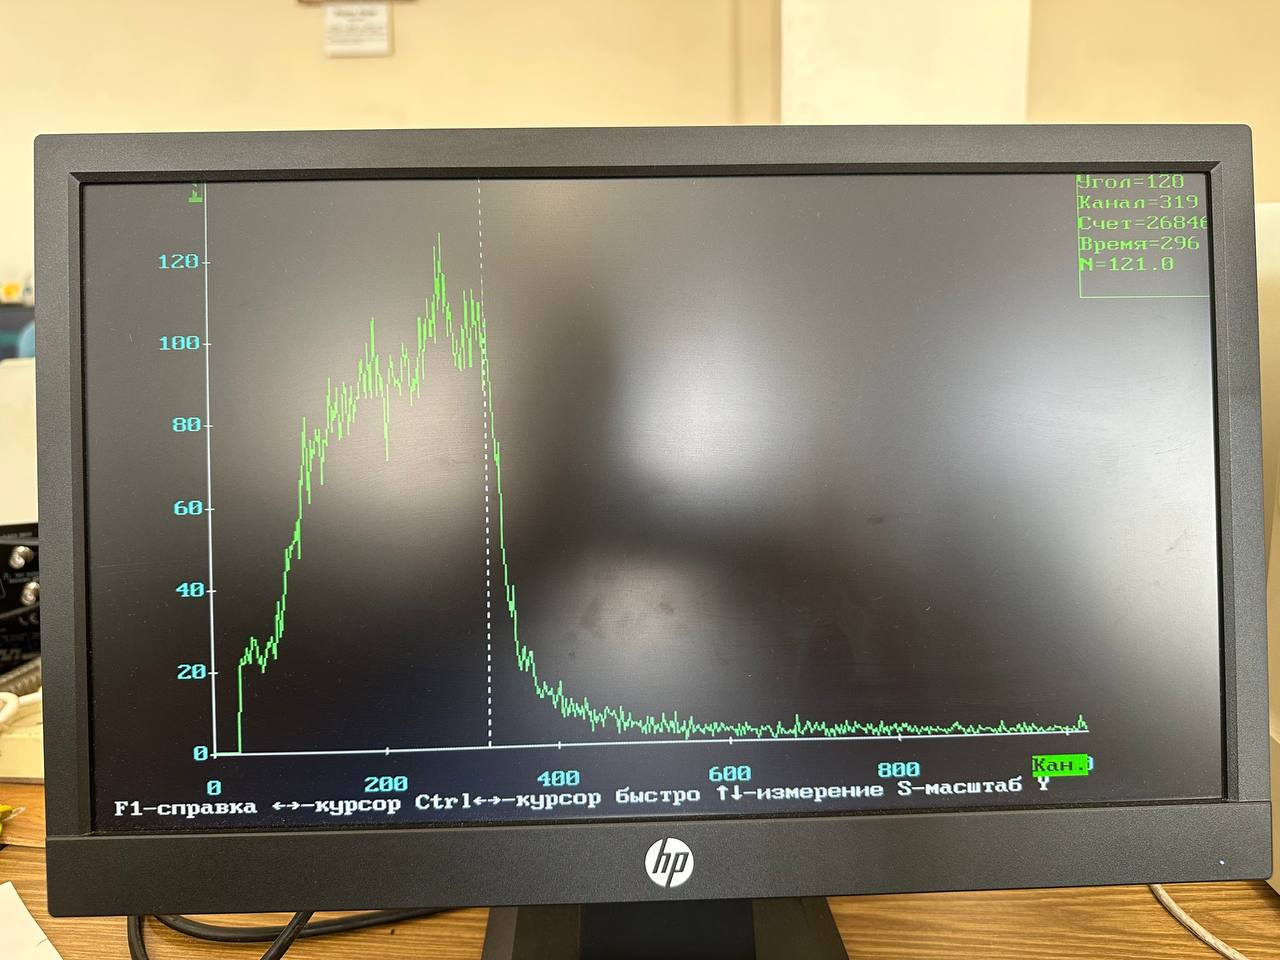
\includegraphics[width = 1\linewidth]{res/013.jpg}
        \caption{$\theta = 120^0$}
        \end{minipage}
    \end{figure}

    Отобразим это все в одной таблице: 
    \begin{figure}[H]
        \centering
        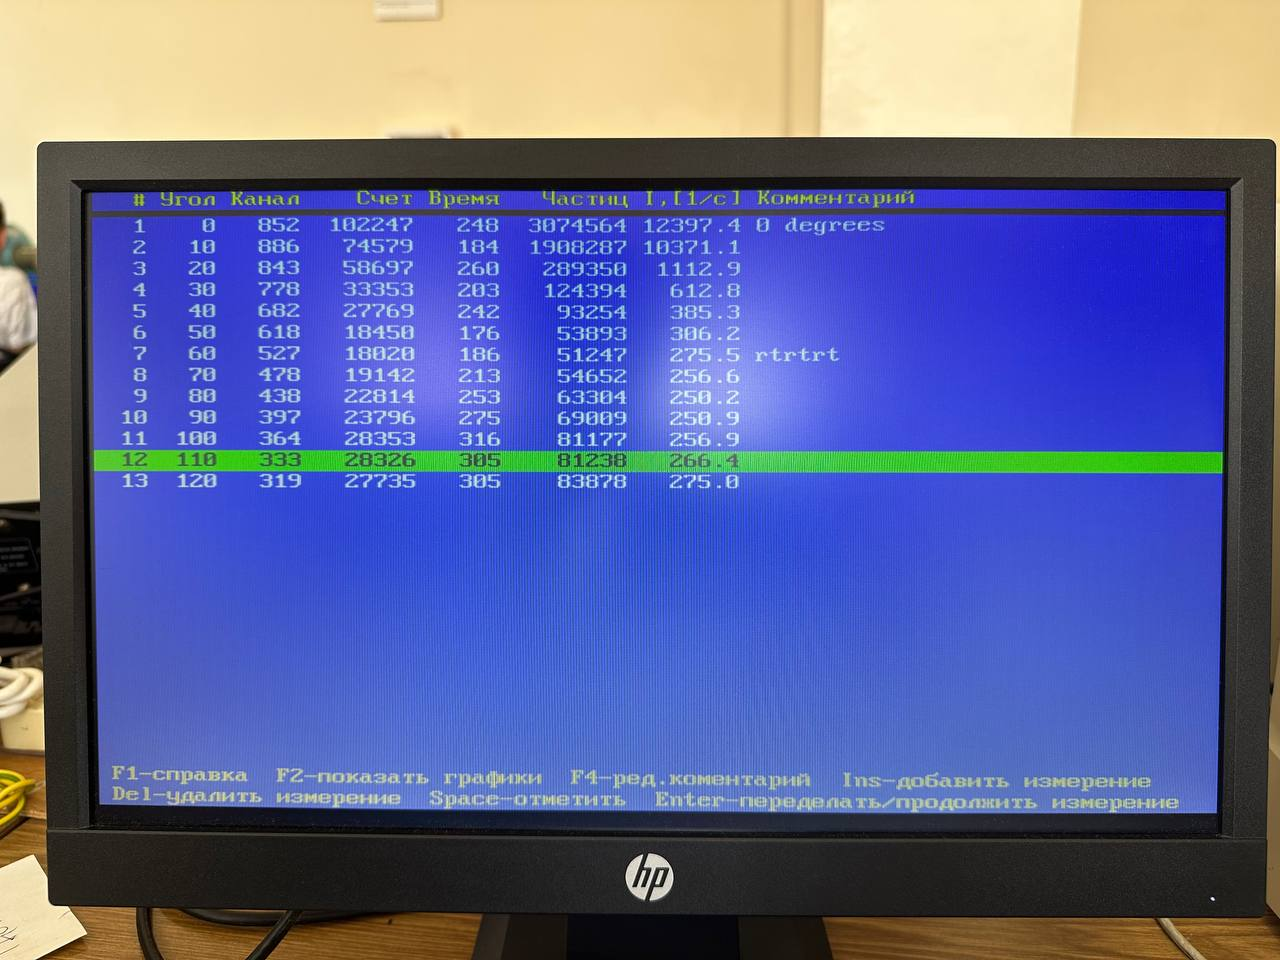
\includegraphics[width=0.7\linewidth]{res/2.jpg}
    \end{figure}

    Теперь построим график, используя формулу (3), откладывая по оси абсцисс $1 - cos \theta$, 
    а по оси ординат величину $1/N(\theta)$:

    \begin{figure}[H]
        \centering
        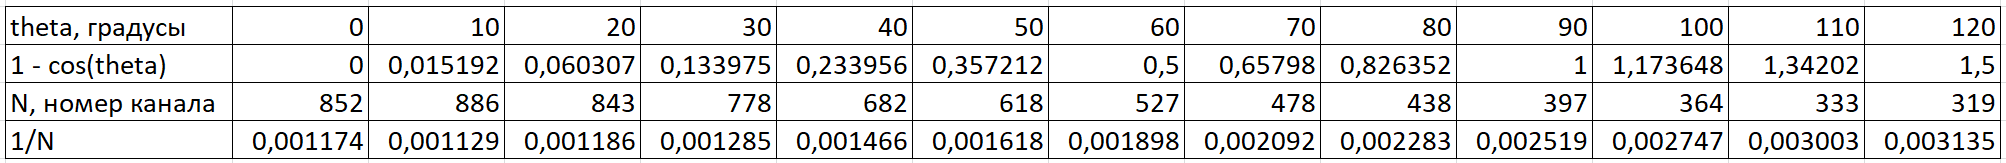
\includegraphics[width=1\linewidth]{res/3.png}
    \end{figure}
    \begin{figure}[H]
        \centering
        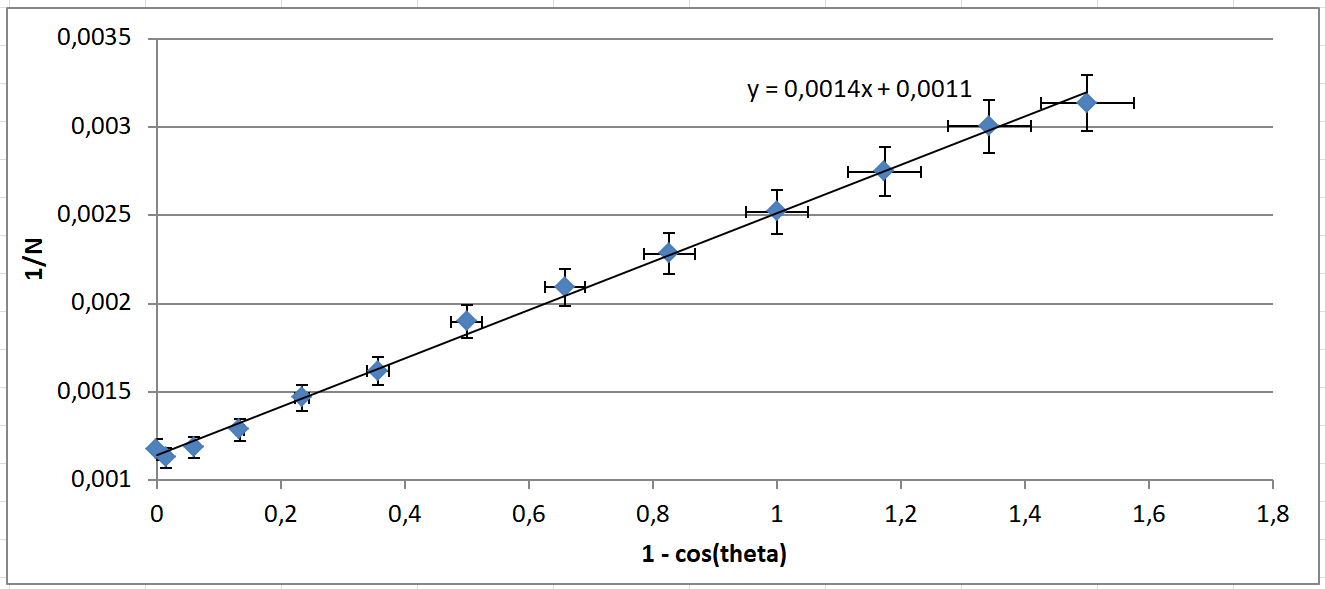
\includegraphics[width=0.7\linewidth]{res/4.png}
    \end{figure}

    С учётом связи между E и N:
    \begin{equation}
        mc^2 (\frac{1}{E(90)} - \frac{1}{E(0)}) = 1
    \end{equation}
    или
    \begin{equation}
        mc^2 = E(0) \frac{E(90)}{E(0) - E(90)} = E_{\gamma} \frac{N(90)}{N(0) - N(90)},
    \end{equation}
    где $E_{\gamma} = 662$ кэВ - энергия налетающего кванта, значение взято из экспериментальной установки.

    Теперь определим энергию покоя частицы, на которой происходит комптоновское рассеяние первичных $\gamma$-частиц,
    используя формулы (4), (5). Для начала определим наилучшие значения N, для углов 90 и 0 градусов:
    \[
        N_{наил}(0) = \dfrac{1}{\dfrac{1}{N(0)}} = \dfrac{1}{0,001142} = 876 \pm 14
    \]
    \[
        N_{наил}(90) = \dfrac{1}{\dfrac{1}{N(90)}} = \dfrac{1}{0,001142 + 0,001371} = 398 \pm 9
    \]

    Тогда:
    \[
        mc^2 = 662*\dfrac{398}{876 - 398} = (551 \pm 11) КэВ
    \]


\section{Заключение}
    В данной работе с помощью сцинтилляционного спектрометра 
    было исследовано энергетическое распределение $\gamma$-квантов, рассеянных на графите. 

    Полученные экспериментальные данные позволили определить энергию рассеянных 
    $\gamma$-квантов в зависимости от угла рассеяния, 
    а также оценить энергию покоя частиц, на которых происходит комптоновское рассеяние. 

\section{Список литературы}
\begin{itemize}
\item Ф. Ф. Игошин, Лабораторный практикум по общей физике. Квантовая физика. Физматкнига, 2012.
\item И. В. Савельев, Курс общей физики: учебное пособие для вуза: в 5 томах. 6-е изд., стер. Т. 1: Механика. Лань, 2021.
\item И. В. Савельев, Курс общей физики. В 5тт. Т. 5 Квантовая оптика. Атомная физика. Физика твердого тела. Физика атомного ядра и элементарных частиц: Учебное пособие. 5-е изд., испр. Лань, 2021.
\item Ю. М. Ципенюк, Кванотовая микро- и макрофизика. Физматкнига, 2006.
\end{itemize}

\end{document}